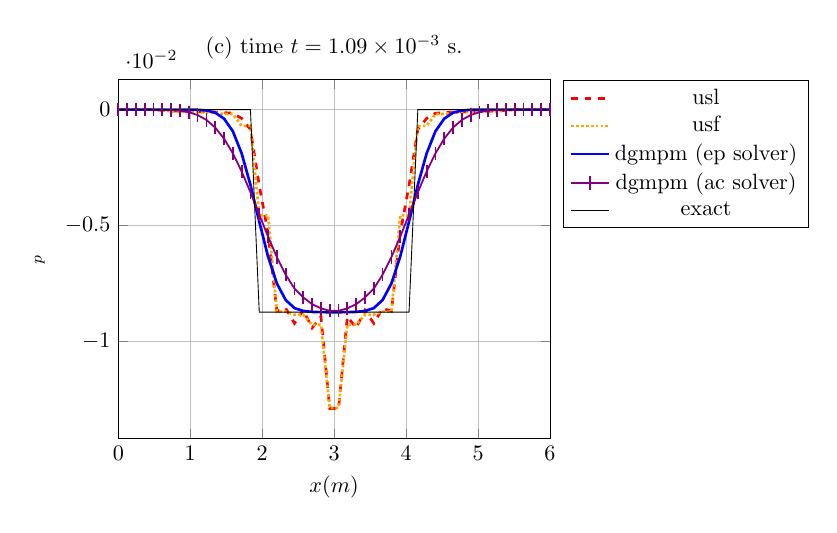
\begin{tikzpicture}[scale=0.8]
\begin{axis}[xlabel=$x (m)$,ylabel=$\eps^p$,ymajorgrids=true,xmajorgrids=true,legend pos=outer north east,title={(c) time $t = 1.09\times 10^{-3} $ s.},xmin=0.,xmax=6.]
\addplot[Red,very thick,mark=none,dashed,mark size=3pt] coordinates {(0.0,0.0) (0.12244897959183673,0.0) (0.24489795918367346,0.0) (0.36734693877551017,0.0) (0.4897959183673469,0.0) (0.6122448979591837,-3.577487902203997e-05) (0.7346938775510203,-6.306588245633642e-05) (0.8571428571428571,-6.949496312549484e-05) (0.9795918367346939,-8.005219978840035e-05) (1.1020408163265305,-9.009475914811774e-05) (1.2244897959183674,-9.858795071160678e-05) (1.346938775510204,-0.00010648019894997112) (1.4693877551020407,-0.00013090237763271645) (1.5918367346938775,-0.00015585484694440393) (1.7142857142857142,-0.00037807434010367157) (1.836734693877551,-0.0008542508721889013) (1.9591836734693877,-0.003265580636192999) (2.0816326530612246,-0.005332403663610279) (2.204081632653061,-0.008685547798871193) (2.326530612244898,-0.008557827562005196) (2.4489795918367347,-0.009212270529983918) (2.571428571428571,-0.008640321746270047) (2.693877551020408,-0.009408157524816411) (2.816326530612245,-0.008914806029937274) (2.9387755102040813,-0.012877303196726952) (3.061224489795918,-0.012877303196726607) (3.183673469387755,-0.008914806029937388) (3.306122448979592,-0.00940815752481628) (3.4285714285714284,-0.008640321746270135) (3.5510204081632653,-0.009212270529983827) (3.673469387755102,-0.008557827562005267) (3.7959183673469385,-0.008685547798871113) (3.9183673469387754,-0.005332403663610266) (4.040816326530612,-0.003265580636192934) (4.163265306122449,-0.0008542508721888987) (4.285714285714286,-0.00037807434010366447) (4.408163265306122,-0.00015585484694441217) (4.530612244897959,-0.00013090237763272187) (4.653061224489796,-0.00010648019894998299) (4.775510204081632,-9.858795071160708e-05) (4.8979591836734695,-9.00947591481104e-05) (5.020408163265306,-8.005219978840008e-05) (5.142857142857142,-6.949496312550109e-05) (5.26530612244898,-6.306588245633955e-05) (5.387755102040816,-3.5774879022040825e-05) (5.5102040816326525,0.0) (5.63265306122449,0.0) (5.755102040816326,0.0) (5.877551020408163,0.0) (6.0,0.0) };
\addplot[Orange,very thick,mark=none,densely dotted,mark size=3pt] coordinates {(0.0,0.0) (0.12244897959183673,0.0) (0.24489795918367346,0.0) (0.36734693877551017,0.0) (0.4897959183673469,-2.538923006910029e-05) (0.6122448979591837,-2.538923006910313e-05) (0.7346938775510203,-8.244814250531935e-05) (0.8571428571428571,-8.244814250532784e-05) (0.9795918367346939,-9.872933660087075e-05) (1.1020408163265305,-9.872933660088494e-05) (1.2244897959183674,-0.0001315062617808007) (1.346938775510204,-0.00013150626178080356) (1.4693877551020407,-0.00019206486011486058) (1.5918367346938775,-0.00019206486011486164) (1.7142857142857142,-0.0007020520949462637) (1.836734693877551,-0.0007020520949463319) (1.9591836734693877,-0.004555064753072419) (2.0816326530612246,-0.004555064753072378) (2.204081632653061,-0.008705849105597185) (2.326530612244898,-0.008705849105596963) (2.4489795918367347,-0.008835786836669598) (2.571428571428571,-0.008835786836669407) (2.693877551020408,-0.009270316426799752) (2.816326530612245,-0.00927031642679947) (2.9387755102040813,-0.012853848358106693) (3.061224489795918,-0.0128538483581062) (3.183673469387755,-0.009270316426799761) (3.306122448979592,-0.00927031642679946) (3.4285714285714284,-0.008835786836669664) (3.5510204081632653,-0.008835786836669336) (3.673469387755102,-0.008705849105597198) (3.7959183673469385,-0.00870584910559694) (3.9183673469387754,-0.004555064753072482) (4.040816326530612,-0.0045550647530723165) (4.163265306122449,-0.0007020520949462988) (4.285714285714286,-0.0007020520949462926) (4.408163265306122,-0.00019206486011485316) (4.530612244897959,-0.00019206486011487072) (4.653061224489796,-0.00013150626178079844) (4.775510204081632,-0.00013150626178081435) (4.8979591836734695,-9.872933660088637e-05) (5.020408163265306,-9.872933660086991e-05) (5.142857142857142,-8.244814250533099e-05) (5.26530612244898,-8.244814250531593e-05) (5.387755102040816,-2.5389230069104546e-05) (5.5102040816326525,-2.538923006909944e-05) (5.63265306122449,0.0) (5.755102040816326,0.0) (5.877551020408163,0.0) (6.0,0.0) };
\addplot[Blue,very thick,mark=none,solid,mark size=3pt] coordinates {(0.0,-5.676632835751488e-19) (0.12244897959183673,-2.3898624238513766e-16) (0.24489795918367346,-3.735990751357306e-14) (0.36734693877551017,-2.3089144911084856e-12) (0.4897959183673469,-7.596762237094698e-11) (0.6122448979591837,-1.5415975357804979e-09) (0.7346938775510203,-2.1087029002110162e-08) (0.8571428571428571,-2.0628580472526095e-07) (0.9795918367346939,-1.5051975779320511e-06) (1.1020408163265305,-8.452232526292688e-06) (1.2244897959183674,-3.741900938747327e-05) (1.346938775510204,-0.00013315210803806102) (1.4693877551020407,-0.00038701776930482674) (1.5918367346938775,-0.0009319386970470464) (1.7142857142857142,-0.0018842066770200564) (1.836734693877551,-0.0032431409441831516) (1.9591836734693877,-0.004827293901207316) (2.0816326530612246,-0.00633202118341673) (2.204081632653061,-0.007489880430691718) (2.326530612244898,-0.008204526972019307) (2.4489795918367347,-0.008552921390073501) (2.571428571428571,-0.008674876019514461) (2.693877551020408,-0.008716486656783273) (2.816326530612245,-0.008726887116624966) (2.9387755102040813,-0.008728580772745199) (3.061224489795918,-0.008728580772745199) (3.183673469387755,-0.008726887116624966) (3.306122448979592,-0.00871648665678328) (3.4285714285714284,-0.008674876019514466) (3.5510204081632653,-0.008552921390073511) (3.673469387755102,-0.008204526972019318) (3.7959183673469385,-0.007489880430691721) (3.9183673469387754,-0.00633202118341673) (4.040816326530612,-0.0048272939012073204) (4.163265306122449,-0.0032431409441831525) (4.285714285714286,-0.001884206677020053) (4.408163265306122,-0.0009319386970470392) (4.530612244897959,-0.0003870177693048181) (4.653061224489796,-0.0001331521080380519) (4.775510204081632,-3.7419009387462476e-05) (4.8979591836734695,-8.452232526284741e-06) (5.020408163265306,-1.5051975779246716e-06) (5.142857142857142,-2.0628580471617835e-07) (5.26530612244898,-2.1087028991608393e-08) (5.387755102040816,-1.5415975312391917e-09) (5.5102040816326525,-7.596762123562041e-11) (5.63265306122449,-2.308913923445202e-12) (5.755102040816326,-3.7358772187005907e-14) (5.877551020408163,-2.4097306387765065e-16) (6.0,-8.514949253627233e-19) };
\addplot[Purple,thick,mark=|,solid,mark size=3pt] coordinates {(0.0,-3.467385013898214e-10) (0.12244897959183673,-6.644251997414089e-09) (0.24489795918367346,-6.120364582198007e-08) (0.36734693877551017,-3.7004598133932975e-07) (0.4897959183673469,-1.6717102054749217e-06) (0.6122448979591837,-6.0577702267402696e-06) (0.7346938775510203,-1.840911253039241e-05) (0.8571428571428571,-4.835925381669828e-05) (0.9795918367346939,-0.00011223737260040385) (1.1020408163265305,-0.00023395773050929446) (1.2244897959183674,-0.0004436331315934306) (1.346938775510204,-0.0007730984959851503) (1.4693877551020407,-0.0012485859668253667) (1.5918367346938775,-0.0018821633869525222) (1.7142857142857142,-0.002664609061018192) (1.836734693877551,-0.003562529161556987) (1.9591836734693877,-0.004521471661696522) (2.0816326530612246,-0.00547485124057479) (2.204081632653061,-0.0063564357486554195) (2.326530612244898,-0.007112831388334339) (2.4489795918367347,-0.00771240428840972) (2.571428571428571,-0.008095314013503907) (2.693877551020408,-0.008383092819259995) (2.816326530612245,-0.008562083426603865) (2.9387755102040813,-0.008669921749349111) (3.061224489795918,-0.008669921749349111) (3.183673469387755,-0.008562083426603865) (3.306122448979592,-0.008383092819260002) (3.4285714285714284,-0.008095314013503904) (3.5510204081632653,-0.007712404288409718) (3.673469387755102,-0.007112831388334339) (3.7959183673469385,-0.006356435748655418) (3.9183673469387754,-0.005474851240574789) (4.040816326530612,-0.004521471661696523) (4.163265306122449,-0.0035625291615569853) (4.285714285714286,-0.0026646090610181854) (4.408163265306122,-0.0018821633869525133) (4.530612244897959,-0.0012485859668253676) (4.653061224489796,-0.0007730984959851409) (4.775510204081632,-0.00044363313159342715) (4.8979591836734695,-0.00023395773050929625) (5.020408163265306,-0.000112237372600403) (5.142857142857142,-4.8359253816693455e-05) (5.26530612244898,-1.8409112530390706e-05) (5.387755102040816,-6.057770226735445e-06) (5.5102040816326525,-1.6717102054752055e-06) (5.63265306122449,-3.7004598133932975e-07) (5.755102040816326,-6.120364582027707e-08) (5.877551020408163,-6.6442519974140885e-09) (6.0,-3.467385011059897e-10) };
\addplot[black,thin,mark=none,solid,mark size=3pt] coordinates {(0.0,-0.0) (0.12244897959183673,-0.0) (0.24489795918367346,-0.0) (0.36734693877551017,-0.0) (0.4897959183673469,-0.0) (0.6122448979591837,-0.0) (0.7346938775510203,-0.0) (0.8571428571428571,-0.0) (0.9795918367346939,-0.0) (1.1020408163265305,-0.0) (1.2244897959183674,-0.0) (1.346938775510204,-0.0) (1.4693877551020407,-0.0) (1.5918367346938775,-0.0) (1.7142857142857142,-0.0) (1.836734693877551,-0.0) (1.9591836734693877,-0.008728715609439695) (2.0816326530612246,-0.008728715609439695) (2.204081632653061,-0.008728715609439695) (2.326530612244898,-0.008728715609439695) (2.4489795918367347,-0.008728715609439695) (2.571428571428571,-0.008728715609439695) (2.693877551020408,-0.008728715609439695) (2.816326530612245,-0.008728715609439695) (2.9387755102040813,-0.008728715609439695) (3.061224489795918,-0.008728715609439695) (3.183673469387755,-0.008728715609439695) (3.306122448979592,-0.008728715609439695) (3.4285714285714284,-0.008728715609439695) (3.5510204081632653,-0.008728715609439695) (3.673469387755102,-0.008728715609439695) (3.7959183673469385,-0.008728715609439695) (3.9183673469387754,-0.008728715609439695) (4.040816326530612,-0.008728715609439695) (4.163265306122449,-0.0) (4.285714285714286,-0.0) (4.408163265306122,-0.0) (4.530612244897959,-0.0) (4.653061224489796,-0.0) (4.775510204081632,-0.0) (4.8979591836734695,-0.0) (5.020408163265306,-0.0) (5.142857142857142,-0.0) (5.26530612244898,-0.0) (5.387755102040816,-0.0) (5.5102040816326525,-0.0) (5.63265306122449,-0.0) (5.755102040816326,-0.0) (5.877551020408163,-0.0) (6.0,-0.0) };
\legend{usl,usf,dgmpm (ep solver),dgmpm (ac solver),exact}
\end{axis}
\end{tikzpicture}
%%% Local Variables:
%%% mode: latex
%%% TeX-master: "../../mainManuscript"
%%% End:
